% Author: Peter von Rohr, peter.vonrohr@gmail.com
% Date: January 18, 2015

\documentclass[11pt,a4paper]{scrartcl}
\usepackage[ngerman]{babel}

\usepackage[T1]{fontenc}      % T1-encoded fonts: auch W?rter mit Umlauten trennen
\usepackage[latin1]{inputenc}

\usepackage{currvita}


\usepackage{relsize}
\usepackage{soul}
\usepackage{xspace}


\usepackage[final]{graphicx}  % um Graphiken einzubinden
%\usepackage{picins} %fuer bild einfuegen
\usepackage{picinpar}


\newcommand{\ccplusplus}{{\sffamily\smaller C/{C}\hbox{\kern.05em\raise.25ex%
  \hbox{+\kern-.01em+}\kern.05em}\spacefactor=1000 }}
\newcommand{\versal}[1]{\textsf{\textsmaller{\MakeUppercase{\caps{#1}}}}\xspace}

\newcommand*{\ac}[1]{\versal{#1}}
\tolerance=600
%%% % make sure everything fits on one page
\textheight=680pt %%% % increase textheight from default 595pt
\pagestyle{empty} %%% % remove pagenumber
\date{}

\begin{document}
%\parpic[rs]{\includegraphics[width=3cm]{bild_sw.jpg}}
\begin{cv}{Curriculum Vitae}

  \setlength{\unitlength}{1pt}
  \begin{picture}(0,0)
  \put(300,-150){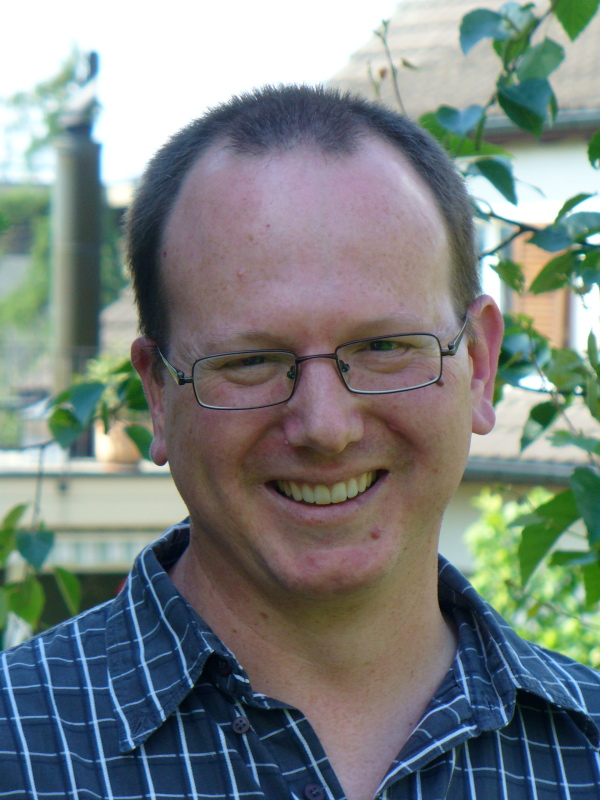
\includegraphics[height=2in]{../pic/portraet600x800}}
  \end{picture}


  \begin{cvlist}{Personal Data}
  \item Peter~von Rohr\\
      St\"ockliackerweg~10\\
      4800~Zofingen
  \item Phone:~062\,751\,54\,65\\
      Mobile:~078\,678\,44\,11\\
      E"~Mail:~peter.vonrohr@gmail.com
  \item Birthdate:~17.\,September\,1968\\
     marital status: in a relationship
  \end{cvlist}
  

  \begin{cvlist}{Education}
  \item[1988--1993] Diploma Study in Agronomy, ETH Zurich
  \item[1993--1998] PhD Study, Economic Values for Growth Performance and Carcass Quality in Pigs, ETH Zurich
  \item[2004--2008] BSc Study in Computer Science, ETH Zurich           
  \end{cvlist}


  \begin{cvlist}{Professional Experience}
  \item[1993--1998]  Assistant, Institute of Animal Science (Animal Breeding) ETH Zurich
  \item[1998--2000]  Postdoc, Departements of Dairy Science and Statistics, Virginia Polytechnic and State University, Blacksburg, USA
  \item[2000--2001]  Lecturer in Pig Breeding, Institute of Animal Science (Animal Breeding) ETH Zurich
  \item[2001--2004]  Oberassistant, Institute of Computational Sciences 
	(Computational Biochemistry Research Group) ETH Zurich
  \item[2008--2011]  IT-Support Engineer and Application Developer, Nebion AG Zurich
  \item[2011--2013]  IT-Support Technician and Project Manager, aargNET GmbH Muhen
  \item[2013--]      Software Developer, Qualitas AG, Zug
  \item[2015--]      Lecturer in Livestock Breeding and Genomics and in Applied Statistical Methods in Animal Science, Institute of Agricultural Science, ETH Zurich
  \item[2016--]      Bioinformatics Internship for next generation sequencing projects, Functional Genomics Center (FGCZ), ETH Zurich and University of Zurich
  \end{cvlist}

  \begin{cvlist}{Further Qualifications}
  \item[Languages] German (mother tongue), English and French
  \end{cvlist}

\pagebreak

  \begin{cvlist}{Computer Skills}
  \item[Operating Systems] Linux, Windows, MacOS
  \item[Programming Languages] R, \ccplusplus, Java, Eiffel, Fortran, 
	Perl, SQL, Matlab, Maple
  \end{cvlist}

  \vspace{-1.5ex}
  \begin{cvlist}{Hobbies}
  \item Folk music, accordeon \vspace{-1ex}
  \item Agriculture, animals, pets and dogs \vspace{-1ex}
  \item Hiking, skiing  \vspace{-1ex}
  \item Singing in the choir Jodler vom Heitere Zofingen\vspace{-1ex}
  \end{cvlist}



%  \cvplace{Zofingen}
%  \date{14.~Mai 2011}

\end{cv}

\end{document}
\endinput
%%
%% End of file
